\pdfminorversion=7
\documentclass[usepdftitle=false, svgnames, color="table, fixpdftex, hyperref, fixinclude, xcdraw", t]{beamer}

\usepackage{lode-i18n}
\usepackage{lode-srccode}
\usepackage{lode-imacid}
\usepackage{lode-pdf}

\usepackage{animate}

\title{Software testing}
\subtitle{Basic concepts}
\author[]{%
Marco Aur�lio Graciotto Silva\inst{1}, \and
Ellen Francine Barbosa\inst{1}, \\\and
M�rcio Eduardo Delamaro\inst{1}, \and
Auri Marcelo Rizzo Vincenzi\inst{2}, \\\and
Jos� Carlos Maldonado\inst{1}}

\newcommand{\numberofinstitutes}{2}
\institute[ICMC]
{
	\inst{1}%
%	\textbf{Institute of Mathematical Sciences and Computing}\\
	University of S�o Paulo (USP)\\
	S�o Carlos, SP, Brazil
	\and
	\inst{2}%
%	\textbf{Institute of Informatics}\\
	Federal University of Goi�s (UFG)\\
	Goi�nia, GO, Brazil
}

\date[]{February 2011}

\logopicture{resources/Logo/icmc-qualipso-inf}

\begin{document}

\frontmatter{}
../CommonAssets/preamble.tex

\mainmatter{}

\part{Software Testing}
\section{Software testing}
\begin{frame}[c, parent={cmap:software-testing}, hasprev=false, hasnext=false]
\frametitle{Software testing}
\label{cmap:software-testing-foundations}

\insertcmap{Courses-SoftwareTesting-BasicConceptsOfSoftwareTesting}
\end{frame}

\subsection{Defect}
\begin{frame}[parent={cmap:software-testing-foundations}, hasprev=false, hasnext=true]
\frametitle{Defect}
\label{concept:defect}

\begin{block:fact}{Defective products}
\begin{itemize}
    \item No product is defect-free.
    \begin{itemize}
		\item And that applies to any kind of product, be it software or
		hardware.
    \end{itemize}
\end{itemize}

\hfill
\refie{example:product-failures}{\beamerbutton{Example: Product failures}}
\end{block:fact}


\begin{block:fact}{Defective software}
\begin{itemize}
	\item No software module is defect-free when implemented and only 40\% of
    software modules are defect-free when released~\cite{shull-etal:2002}.
\end{itemize}
\hfill
\refie{example:software-failures}{\beamerbutton{Example: Software failures}}
\end{block:fact}
\end{frame}


\begin{frame}[hasprev=true, hasnext=true]
\frametitle{Defect}
\label{concept:defect-detection}

\begin{block:fact}{Every software has defects}
\begin{itemize}
	\item Even small, simple, trivial products are error-prone.
\end{itemize}
\end{block:fact}

\begin{block}{Example: Triangle}
\centering
\refie{example:triangle}{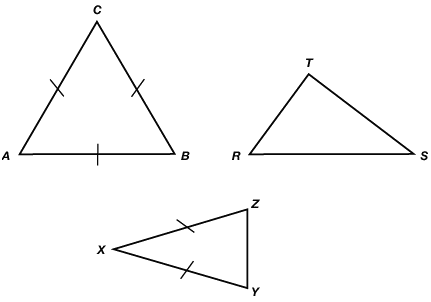
\includegraphics[scale=.5]{resources/Triangle/Equilateral-Isosceles-Scalene-triangles}}
\end{block}
\end{frame}


\begin{frame}[hasprev=true, hasnext=false]
\frametitle{Defect}

\begin{block:fact}{Defect avoidance and detection}
\begin{itemize}
	\item Nevertheless, products failures could and must be avoided and
	corrected, as they negatively impacts software quality.
\end{itemize}
\end{block:fact}


\begin{block:fact}{Why we should care about it?}
\begin{itemize}
    \item Rising demand for higher software quality.

    \item Software defect reduction improves software quality.
\end{itemize}
\end{block:fact}

\begin{block:fact}{Software quality and software testing}
\begin{itemize}
	\item The main goal of software testing is to find defects.

	\item Systematic software testing, carried out using proper techniques,
	criteria, and tools, improves software reliability (and quality).
\end{itemize}
\end{block:fact}
\end{frame}


\subsection{Software testing}
\begin{frame}[c, parent={cmap:software-testing}, hasprev=false, hasnext=false]
\frametitle{Software testing}
\label{cmap:software-testing-foundations}

\insertcmap{Courses-SoftwareTesting-BasicConceptsOfSoftwareTesting}
\end{frame}

\subsection{Defect taxonomy}
\begin{frame}[parent={cmap:software-testing-foundations}, hasprev=false, hasnext=true]
\frametitle{Defect taxonomy}
\framesubtitle{Fault}
\label{concept:fault}

\begin{block:concept}{What is a fault?}
A fault is an incorrect data definition, step, or process in a software.
\end{block:concept}

\begin{block:fact}{How a fault is created?}
\begin{itemize}
	\item A fault is inserted by a mistake.
\end{itemize}
\end{block:fact}

\hfill
\refie{example:incorrect-statement-2}{\beamerbutton{Example: Incorrect statement}}
\end{frame}



\begin{frame}[hasprev=true, hasnext=true]
\label{concept:mistake}
\frametitle{Defect taxonomy}
\framesubtitle{Mistake}

\begin{block:concept}{What is a mistake?}
A mistake is a human action that produces an incorrect result.
\end{block:concept}

\begin{block:fact}{How a mistake takes place?}
\begin{itemize}
	\item Lack of attention when implementing the software?

	\item Omitted information in the software requirement specification?

	\item Compiler fault (which by itself was caused by a mistake)?
\end{itemize}
\end{block:fact}

\hfill
\refie{example:incorrect-statement-1}{\beamerbutton{Example: Incorrect statement}}
\end{frame}



\begin{frame}
\label{concept:error}
\frametitle{Defect taxonomy}
\framesubtitle{Error}

\begin{block:concept}{What is an error?}
An error is the difference between a computed, observed or measured value
or condition and the true, theoretically correct or specified value or
condition.
\end{block:concept}

\begin{block:fact}{How an error occurs?}
\begin{itemize}
	\item An error is produced by the execution of a fault.
	\begin{itemize}
		\item Thus, if a fault is never executed, it never produces an error.
	\end{itemize}
\end{itemize}
\end{block:fact}
\end{frame}


\begin{frame}
\label{concept:failure}
\frametitle{Defect taxonomy}
\framesubtitle{Failure}

\begin{block:concept}{What is a failure?}
A failure is the inability of a component or a system to fulfill its
required functions within specified performance requirements.
\end{block:concept}

\begin{block:fact}{How a failure occurs?}
\begin{itemize}
	\item A fault and its associated errors may cause one or more failures.
\end{itemize}
\end{block:fact}

\hfill
\refie{example:incorrect-statement-3}{\beamerbutton{Example: Incorrect statement}}
\end{frame}



\begin{frame}
\frametitle{Defect taxonomy}

\begin{block:procedure}{Summary}
\begin{enumerate}
	\item A programmer makes a \textbf{mistake}.
	\begin{itemize}
		\item One single $<$ is replaced by a $>$ in a single statement.
	\end{itemize}

	\item Due to the mistake, the statement is \textbf{faulty} (it does
	not implement the behavior described in the software requirements
	specification).

	\item The software is compiled and run. The given statement is run. As it
	belongs to a function in charge of creating the checksum of the data being
	processed, the output is produces is incorrect (\textbf{error}).

	\item The user compares the checksum produces by the software with the
	expected one. No matter what, the checksum always \textbf{fails}.
\end{enumerate}
\end{block:procedure}
\end{frame}



\begin{frame}[c, hasprev=true, hasnext=false]
\label{concept:defect-taxonomy}
\frametitle{Defect taxonomy}

\begin{block:fact}{}
    \centering
    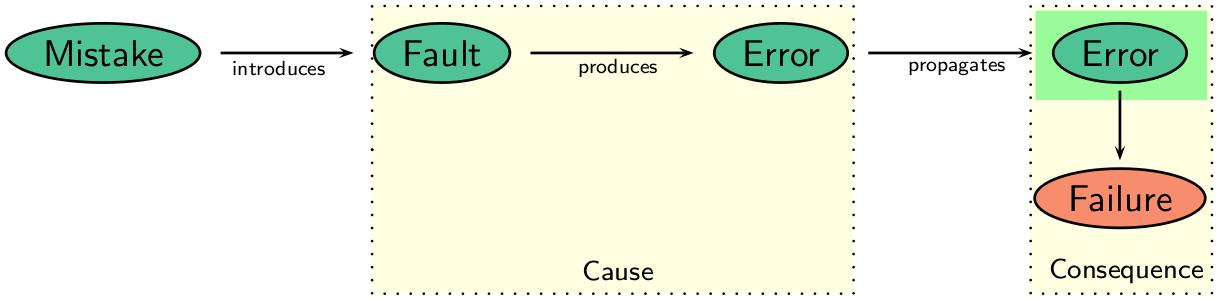
\includegraphics[scale=.3]{defect-taxonomy}
\end{block:fact}

\hfill
\refie{example:physician-analogy-for-defect-taxonomy}{\beamerbutton{Example: Physician analogy for defect taxonomy}}
\refie{example:numzero}{\beamerbutton{Example: Defect taxonomy example (numZero)}}
\end{frame}


\subsection{Test case}
\begin{frame}[parent={cmap:jabuti-gui},hasnext=true,hasprev=true]
\frametitle{Main functionalities}
\framesubtitle{Test Case Menu}
\label{concept:test-case-menu}

\begin{block}{Test case}
The \highlight{Test Case} menu provides options for test set manipulation and
report generation.
\end{block}

\begin{block}{Demo}
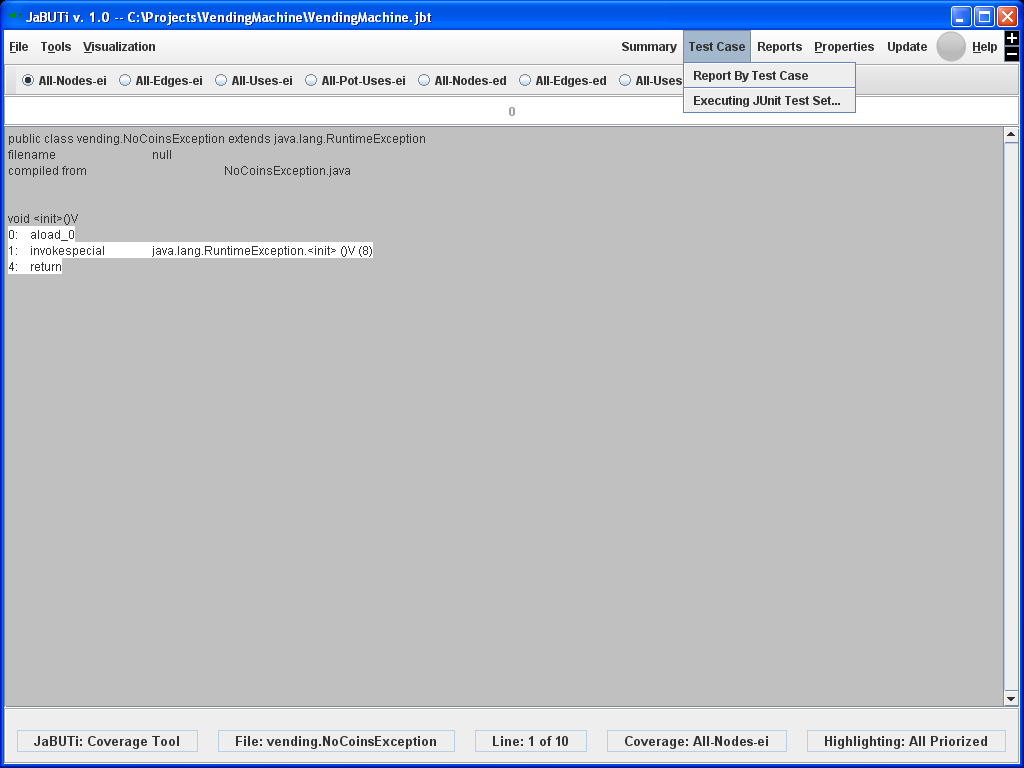
\includegraphics[width=\textwidth,clip]{resources/JaBUTi/JaBUTi-GUI/JaBUTi-GUI-TestCase/JaBUTi-GUI-TestCase}
\end{block}
\end{frame}



\begin{frame}
\frametitle{Main functionalities}
\framesubtitle{Test Case Menu}
\label{concept:report-by-test-case}

\begin{block}{Report By Test Case}
\highlight{Report By Test Case} option shows the coverage information with
respect to the current selected test criterion, for each individual test case,
considering all class under testing, and also allows to enable/disable and
delete/undelete test cases.
\end{block}

\begin{block}{Demo}
\insertmovie{JaBUTi/JaBUTi-GUI/JaBUTi-GUI-TestCase-ReportByTestCase/JaBUTi-GUI-TestCase-ReportByTestCase}
\end{block}
\end{frame}



\begin{frame}
\frametitle{Main functionalities}
\framesubtitle{Test Case Menu}
\label{concept:importing-from-junit}

\begin{block}{Importing from JUnit}
\highlight{Importing from JUnit} option allows to import a test set generated
according to the JUnit framework.
\end{block}

\begin{block}{Demo}
\insertmovie{JaBUTi/JaBUTi-GUI/JaBUTi-GUI-TestCase-ExecutingJUnitTestSet/JaBUTi-GUI-TestCase-ExecutingJUnitTestSet}
\end{block}
\end{frame}


\subsection{Oracle}
\begin{frame}[parent={cmap:software-testing},hasnext=true,hasprev=true]
\label{concept:oracle}
\frametitle{Oracle}

\begin{block:concept}{Definition}
An oracle is any software, process, or data that provides the test designer
with the expected result of a test case.
\end{block:concept}

\begin{block:fact}{}
\begin{itemize}
	\item An oracle decides whether output values are correct against what is
	specified.
	\begin{itemize}
		\item An oracle is required to determine whether a fault was revealed.
	\end{itemize}

	% TODO: Propose a better classification of oracles
	\item Some examples of oracle: human guess (kiddie oracle), regression
	test suite, validated data, purchased test suite, existing software.
\end{itemize}
\end{block:fact}
\end{frame}



\begin{frame}
\label{concept:kiddie-oracle}
\frametitle{Oracle}
\framesubtitle{Kiddie oracle}

\begin{block:concept}{Definition}
A kiddie oracle is obtained from running the software and seeing the output. If
it looks about right, it must be right.
\end{block:concept}

\begin{block:fact}{Why should I use a kiddie oracle?}
\begin{itemize}
	\item Actually, you should not use it, as its very error prone.

	\item Nonetheless, it is better than nothing.
	\begin{itemize}
		\item And, if the expected behavior of the application is not
		documented, it is up to the user to detect the correct result anyway.
	\end{itemize}
\end{itemize}
\end{block:fact}


\hfill
\refie{example:kiddie-oracle}{\beamerbutton{Example: Human guess (kiddie) oracle}}
\end{frame}



\begin{frame}
\label{concept:regression-test-suite-oracle}
\frametitle{Oracle}
\framesubtitle{Regression test suite oracle}

\begin{block:concept}{Definition}
A regression test suite oracle  is obtained from running the test case and
comparing the output to the results of the same test cases run against a
previous version of the software.
\end{block:concept}

\begin{block:fact}{Why should I use a regression suite oracle?}
\begin{itemize}
	\item Regression test ensures that the modified system functions as per
	its specification.

	\item It ensures that old errors will not appear again (or that, at least,
	they will be detected earlier).
\end{itemize}
\end{block:fact}


\hfill
\refie{example:mozilla-firefox-regression-test-suite-oracle}{\beamerbutton{Example: Regression test suite oracle for Mozilla Firefox}}
\end{frame}



\begin{frame}
\label{concept:purchased-test-suite-oracle}
\frametitle{Oracle}
\framesubtitle{Purchased test suite oracle}

\begin{block:concept}{Definition}
A purchased test suite oracle consists in running the software against a
standardized test suite that has been previously created and validated.
\end{block:concept}

\begin{block:fact}{Why should I use a purchased oracle?}
\begin{itemize}
	\item Usually it is required that a software passes a test suite oracle
	in order assess its compliance to a particular technology or standard.

	\item Sometimes its simply easier to buy a test suite instead of developing
	your own.
\end{itemize}
\end{block:fact}


\hfill
\refie{example:java-test-suite-oracle}{\beamerbutton{Example: Java TCK}}
\end{frame}


\subsection{Test phase}
\begin{frame}[parent={cmap:software-testing-foundations}, hasprev=false, hasnext=true]
\frametitle{Test phases}

\begin{block:fact}{What I should test first?}
\begin{itemize}
	\item What should I target when testing a software?

	\item The definition of a single target for each test activity is key for
	systematic software testing.
	\begin{itemize}
		\item Focus effort and restrict available techniques (thus lowering
		costs and, probably, increasing efficacy).
	\end{itemize}

	\item A common sense approach would be to begin testing the smallest
	module possible, and then proceed to test the interactions between these
	modules and, finally, the system as a whole.
\end{itemize}
\end{block:fact}
\end{frame}


\begin{frame}[hasprev=true, hasnext=true]
\frametitle{Test phases}
\label{concept:test-phase}
\label{concept:phase}

\begin{block:concept}{Definition}
Test phase is a categorization of test activities which is directly related
to the software life cycle the activities take place in.
\end{block:concept}

\begin{block:fact}{Definitions}
\begin{itemize}
	\item Test phases allow the tester to concentrate on various aspects of
	the software and use different test criteria at each one.

	\item Test activities are organized in test phases such that testing starts
	with the smallest executable unit until reaching the software as a whole:
	\begin{itemize}
		\item Unit testing.
		\item Integration testing.
		\item System testing.
		\item Acceptance testing.
	\end{itemize}
\end{itemize}
\end{block:fact}
\end{frame}


\begin{frame}[c]
\frametitle{Test phases}

\begin{figure}
    \centering
    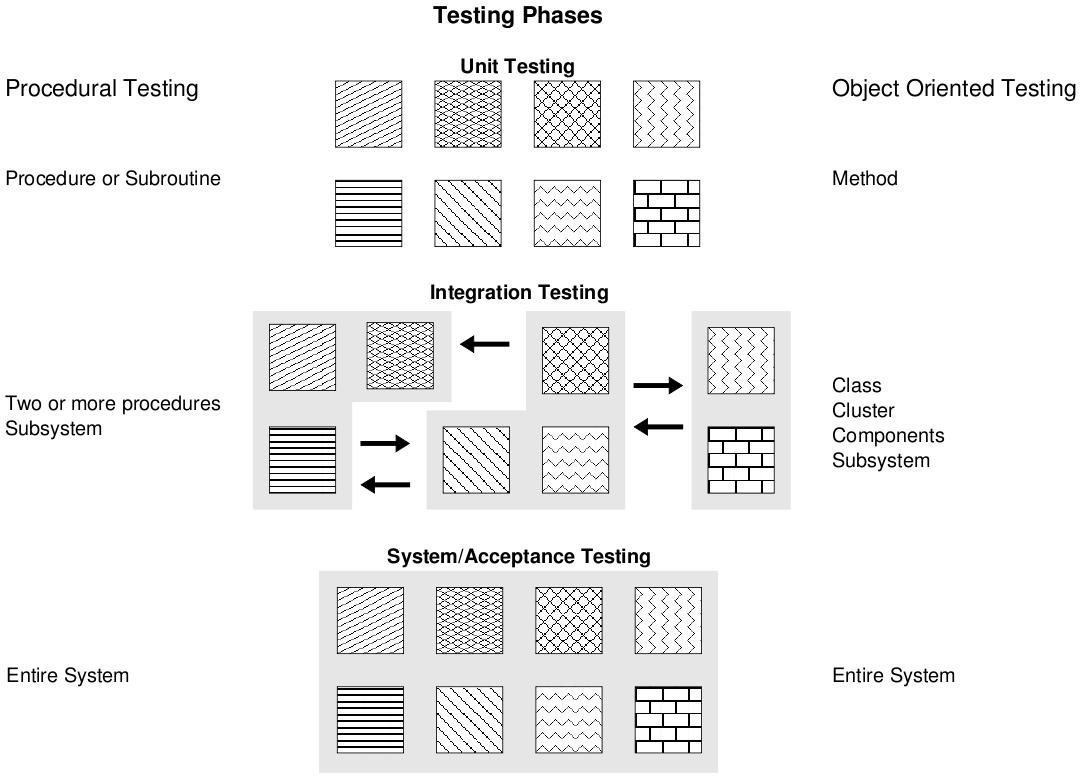
\includegraphics[scale=.3]{figs/test-phases}
\end{figure}
\end{frame}


\begin{frame}
\frametitle{Test phases}
\framesubtitle{Unit testing}
\label{concept:unit-testing}

\begin{block:concept}{Definition}
Unit testing verifies the functioning in isolation of software pieces which
are separately testable.
\end{block:concept}

\begin{figure}
    \centering
    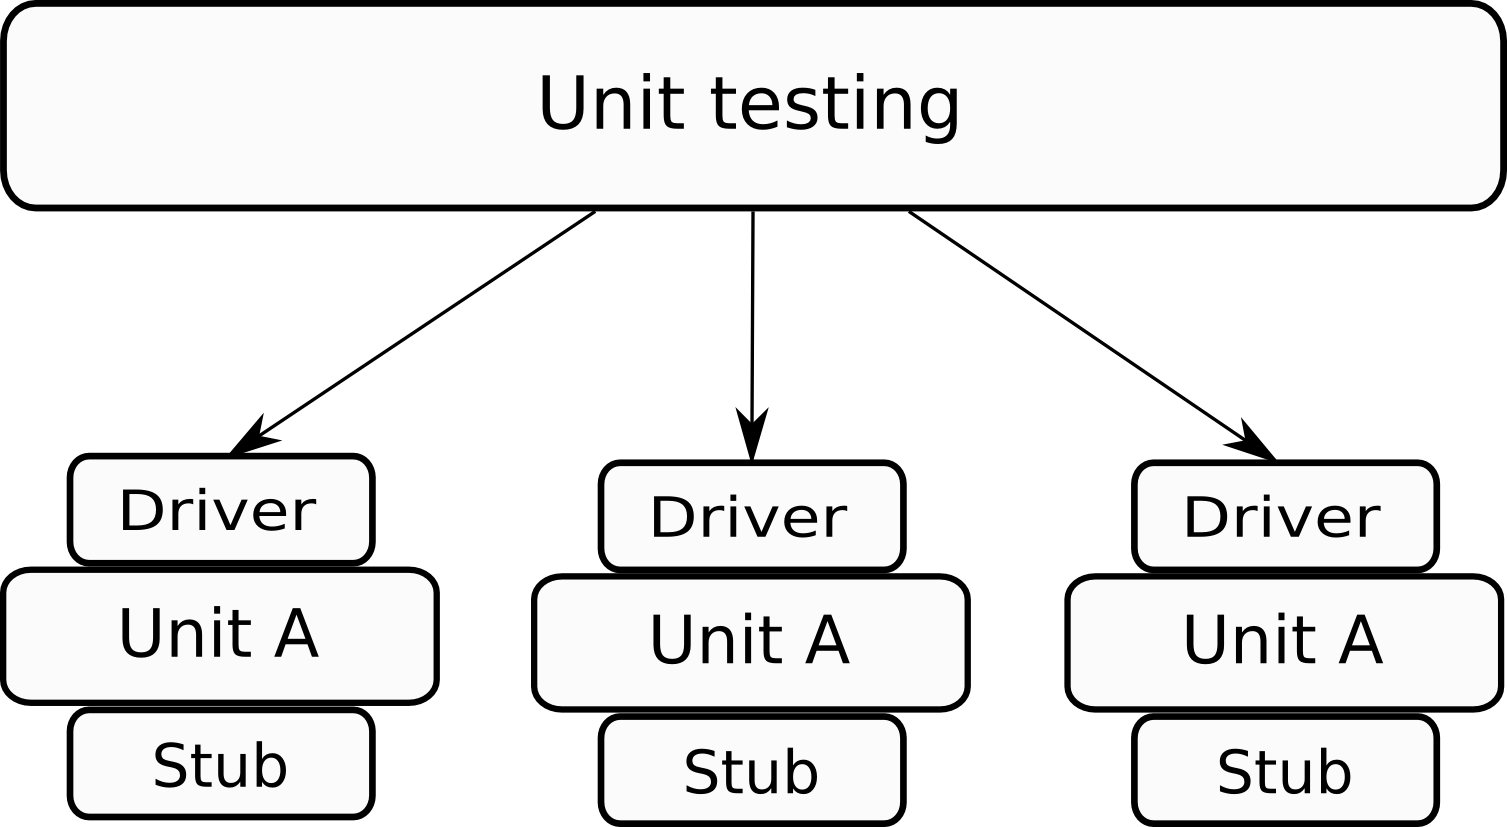
\includegraphics[width=5cm]{figs/unit-testing}
\end{figure}

\hfill
\refie{example:pentium-fdiv-bug}{\beamerbutton{Example: Pentium FDIV bug}}
\end{frame}


\begin{frame}
\frametitle{Test phases}
\framesubtitle{Unit testing}

\begin{block:fact}{What is an unit?}
\begin{itemize}
	\item In procedural testing, the unit is the procedure or subroutine.

	\item In object oriented testing, the unit is the method or the class.
	\begin{itemize}
		\item For the time being, we will consider that the unit is the method!
	\end{itemize}
\end{itemize}
\end{block:fact}
\end{frame}



\begin{frame}
\frametitle{Test phases}
\framesubtitle{Unit testing - Stubs}

\begin{block:fact}{How to test an unit?}
\begin{itemize}
	\item Although the definition calls for units that are separately testable,
	this is not always possible.
	\begin{itemize}
		\item Mosts units requires data from other units.
	\end{itemize}

	\item Coupling between units is a threat for unit testing. Thus, it is
	desirable to replace some units by others more simple and predictable
	(just for software testing sake).
\end{itemize}
\end{block:fact}
\end{frame}



\begin{frame}
\frametitle{Test phases}
\framesubtitle{Stubs}
\label{concept:stub}

\begin{block:concept}{Definition}
A stub is a unit that replaces another unit used by the unit under test.
\end{block:concept}

\begin{block:fact}{Why should we use a stub?}
\begin{itemize}
	\item Stubs simulate the behavior of another unit not yet implemented but
	called by the unit under test.

	\item Usually, a stub simulates the expected behavior of the used unit with
	minimum computation effort or data manipulation.
\end{itemize}
\end{block:fact}

\hfill
\refie{example:stub}{\beamerbutton{Example: Stub}}
\end{frame}


\begin{frame}
\frametitle{Test phases}
\framesubtitle{Unit testing - Driver}

\begin{block:fact}{How to test a unit?}
\begin{itemize}
	\item Even tough stubs can be used to replace complex units for a given
	unit under testing, something must setup and wire the stubs into the
	unit.
\end{itemize}
\end{block:fact}
\end{frame}



\begin{frame}
\frametitle{Test phases}
\framesubtitle{Unit testing - Driver}
\label{concept:driver}
\label{concept:test-driver}

\begin{block:concept}{Definition}
Driver is the software responsible for coordinating the testing of a unit.
\end{block:concept}

\begin{block:fact}{What a driver does?}
\begin{itemize}
	\item Drivers are used to test a unit which requires input data provided
	by another unit:
	\begin{enumerate}
		\item it gathers the data provided by the tester,
		\item it passes them to the unit under test in the form of arguments,
		\item it collects the results produced by the unit, and
		\item it shows them to the tester.
	\end{enumerate}
\end{itemize}
\end{block:fact}
\end{frame}


\begin{frame}[c]
\frametitle{Test phases}
\framesubtitle{Unit testing - Driver and stubs}

\begin{figure}
	\centering
	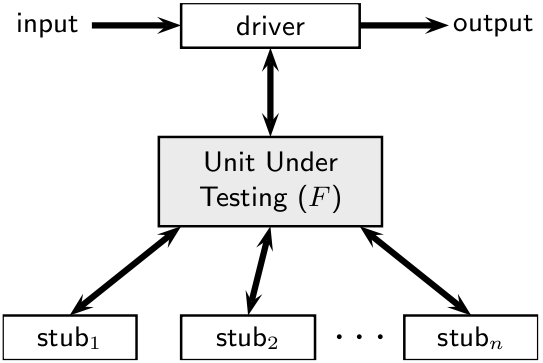
\includegraphics[scale=.3]{figs/driver-and-stub}
\end{figure}
\end{frame}



\begin{frame}
\label{concept:integration-testing}
\frametitle{Test phases}
\framesubtitle{Integration testing}

\begin{block:concept}{Definition}
Integration testing verifies whether the units tested individually communicate
accordingly when integrated.
\end{block:concept}

\begin{figure}
    \centering
    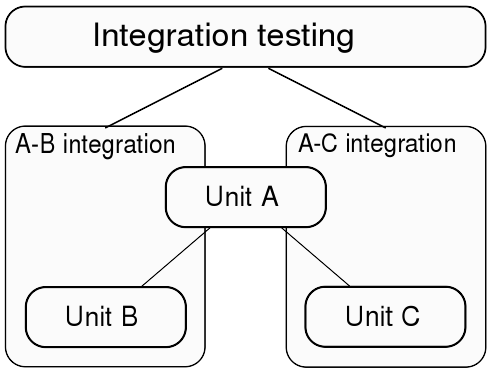
\includegraphics[scale=.3]{figs/integration-testing}
\end{figure}

\hfill
\refie{example:mars-climate-orbiter}{\beamerbutton{Example: Mars climate orbiter}}
\end{frame}



\begin{frame}
\frametitle{Test phases}
\framesubtitle{Integration testing}

\begin{block:fact}{Why integration testing is important?}
\begin{itemize}
	\item Integration testing must be performed because:
	\begin{itemize}
		\item Data can be lost at the unit's interface.

		\item Global variables can suffer undesirable interferences.
	\end{itemize}
\end{itemize}
\end{block:fact}

\begin{figure}
    \centering
    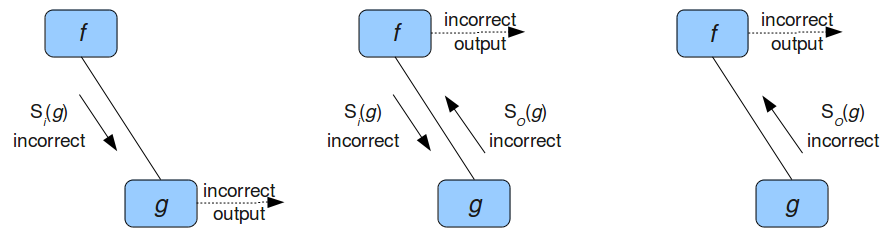
\includegraphics[width=\textwidth]{figs/types-integration-errors}
\end{figure}
\end{frame}


\begin{frame}
\label{concept:system-testing}
\frametitle{Test phases}
\framesubtitle{System testing}

\begin{block:concept}{Definition}
System testing ensures that the software and the other elements that
are part of the system (hardware and database, for instance) are adequately
combined and behave as expected.
\end{block:concept}

\begin{block:fact}{Types of system testing}
\begin{itemize}
	\item Typically system testing includes many types of testing:
	\begin{columns}[t, totalwidth=6.5cm]
		\begin{column}[t]{3cm}
			\begin{itemize}
				\item functionality,
				\item usability,
				\item security,
				\item localization,
			\end{itemize}
		\end{column}

		\begin{column}[t]{3cm}
			\begin{itemize}
				\item reliability,
				\item availability,
				\item \ldots
			\end{itemize}
		\end{column}
	\end{columns}
\end{itemize}
\end{block:fact}

\hfill
\refie{example:ghost-train}{\beamerbutton{Example: Ghost train}}
\end{frame}



\begin{frame}[hasprev=true, hasnext=false]
\label{concept:acceptance-testing}
\frametitle{Test phases}
\framesubtitle{Acceptance testing}

\begin{block:concept}{Definition}
Acceptance testing refers to the tester, in general performed by the
user himself, who verifies whether the product satisfies his expectation.
\end{block:concept}

\begin{block:fact}{Alpha/Beta testing}
\begin{itemize}
	\item Informally, it can be defined alpha and beta testing.
	\begin{itemize}
		\item Alpha testing: software is installed and used internally (in the
		company that developed).

		\item Beta testing: software is installed and tested by external
		users.
	\end{itemize}
\end{itemize}
\end{block:fact}

\begin{block:fact}{Why is acceptance testing important?}
\begin{itemize}
    \item Acceptance testing, when completed successfully, will result in the
    customer accepting the software.
\end{itemize}
\end{block:fact}
\end{frame}

\subsection{Test criterion}
\begin{frame}[parent={cmap:software-testing},hasnext=true,hasprev=true]
\label{concept:test-criterion}
\frametitle{Test criterion}

\begin{block:concept}{Definition}
A test criterion systematizes the way test requirements are
generated from the source of information (specification, source code,
historical fault database, etc.).
\end{block:concept}

\begin{block:fact}{}
\begin{itemize}
	\item A test criterion provides a systematic way to select test cases.
	\begin{itemize}
		\item A testing criterion divides the input domain.
	\end{itemize}

	\item When no faults are found, test criterion provides an indication of
	how test cases should be selected in order to establish a high level of
	confidence of product correction.
\end{itemize}
\end{block:fact}

\hfill
\refie{example:test-criterion}{\beamerbutton{Example: Test criterion example}}
\end{frame}


\begin{frame}
\frametitle{Test criterion}

\begin{block:fact}{Test criterion attributes}
\begin{itemize}
	\item A test criterion can be compared based on cost, efficacy and
	strength.
\end{itemize}
\end{block:fact}

\begin{figure}
    \centering
    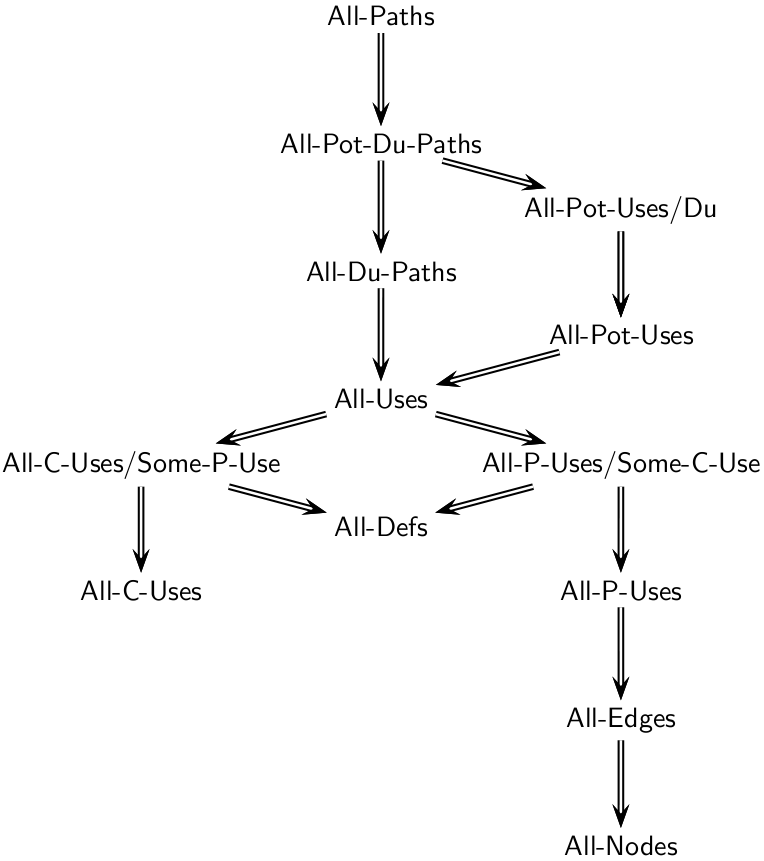
\includegraphics[width=4cm]{subsume-relation}
\end{figure}
\end{frame}


\subsection{Test requirement}
\begin{frame}[parent={cmap:software-testing-foundations}, hasprev=false, hasnext=true]
\frametitle{Test requirement}
\label{concept:test-requirement}

\begin{block:concept}{Definition}
A test requirement is a specific element of a software artifact that a test
case must satisfy or cover.
\end{block:concept}

\begin{block:fact}{How a test requirement is created?}
\begin{itemize}
	\item Test requirements are derived from the program under testing using
	a specific test criterion.
\end{itemize}
\end{block:fact}

\begin{block:fact}{What are test requirements for?}
\begin{itemize}
	\item A test requirement can:
	\begin{itemize}
		\item evaluate a test set, and
		\item generate a test set.
	\end{itemize}
\end{itemize}
\end{block:fact}
\end{frame}


\begin{frame}[hasprev=true, hasnext=false]
\label{concept:test-set}
\label{concept:c-adequate-test-set}
\frametitle{Test requirement}
\framesubtitle{Test set}

\begin{block:concept}{Definition}
A test set is a set of test cases.
\end{block:concept}

\begin{block:fact}{Test sets and test requirements}
\begin{itemize}
	\item A test set can be improved by adding test cases that exercise
	uncovered requirements.
	\begin{itemize}
		\item The best test set is the smallest one that indicates the largest
		set of faults.
	\end{itemize}
\end{itemize}
\end{block:fact}

\begin{block:concept}{C-adequate test sets}
\begin{itemize}
	\item When a test set $T$ satisfies all the test requirements derived from
	a program using a given criterion $C$, $T$ is said $C-adequate$.
\end{itemize}
\end{block:concept}
\end{frame}

\subsection{Test technique}
\begin{frame}[parent={cmap:software-testing-foundations}, hasprev=false, hasnext=true]
\frametitle{Test technique}
\label{concept:test-technique}

\begin{block:concept}{Definition}
Test techniques are types of testing defined according to the
source of information used to carried out the testing activity.
\end{block:concept}

\begin{block:fact}{Test techniques and test criteria}
\begin{itemize}
    \item Each test technique has a set of associated test criteria.
\end{itemize}
\end{block:fact}
\end{frame}



\begin{frame}[hasprev=true, hasnext=true]
\frametitle{Test technique}

\begin{block:fact}{Software test techniques}
\begin{itemize}
	\item Exhaustive testing

	\item Random testing

	\item Partition testing
	\begin{itemize}
		\item Fault-based testing

		\item Functional testing

		\item Structural testing
	\end{itemize}
\end{itemize}
\end{block:fact}
\end{frame}



\begin{frame}
\frametitle{Test technique}
\framesubtitle{Exhaustive testing}
\label{concept:exhaustive-testing}

\begin{block:concept}{Definition}
An exhaustive test executes the software with all possible value from its
input domains.
\end{block:concept}

\begin{block:fact}{}
    \centering
    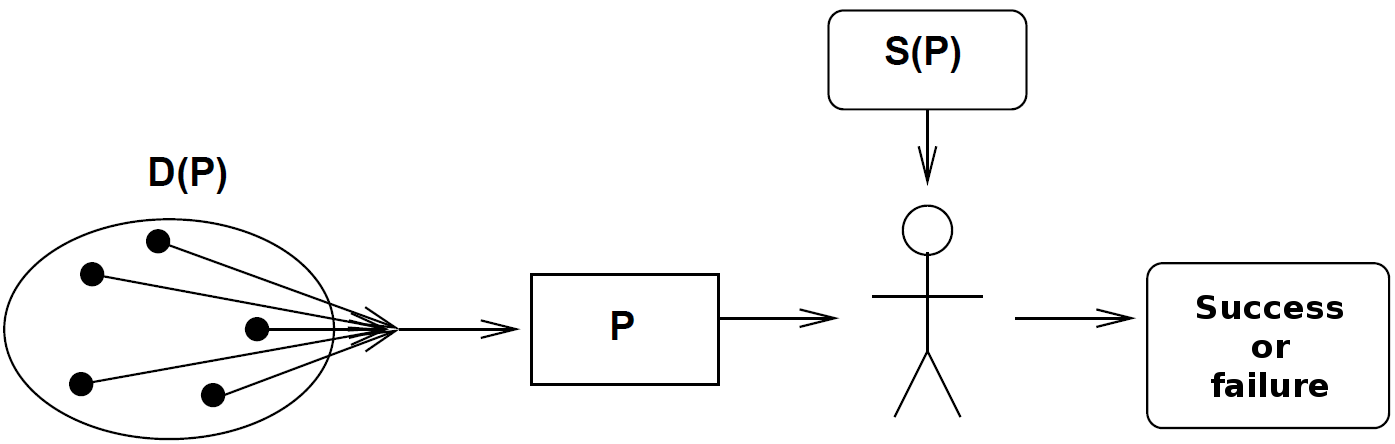
\includegraphics[width=\textwidth]{exhaustive-software-testing}
\end{block:fact}

\hfill
\refie{example:blech-exhaustive-testing}{\beamerbutton{Example: Exhaustive testing of the blech function}}
\end{frame}



\begin{frame}
\frametitle{Test technique}
\framesubtitle{Exhaustive testing}

\begin{block:fact}{Exhaustive testing limitations}
\begin{itemize}
	\item Can be prohibitive due to time and cost constraints for finite
	but large input domain.

	\item Impossible if the input domain is infinite.

	\item Infeasible in general.
\end{itemize}
\end{block:fact}
\end{frame}



\begin{frame}
\frametitle{Test technique}
\framesubtitle{Random testing}
\label{concept:random-testing}

\begin{block:concept}{Definition}
Random testing uses a systematic method to generate test cases: it
requires modeling the input space and then sampling data from the input
space randomly.
\end{block:concept}

\begin{block:fact}{}
    \centering
    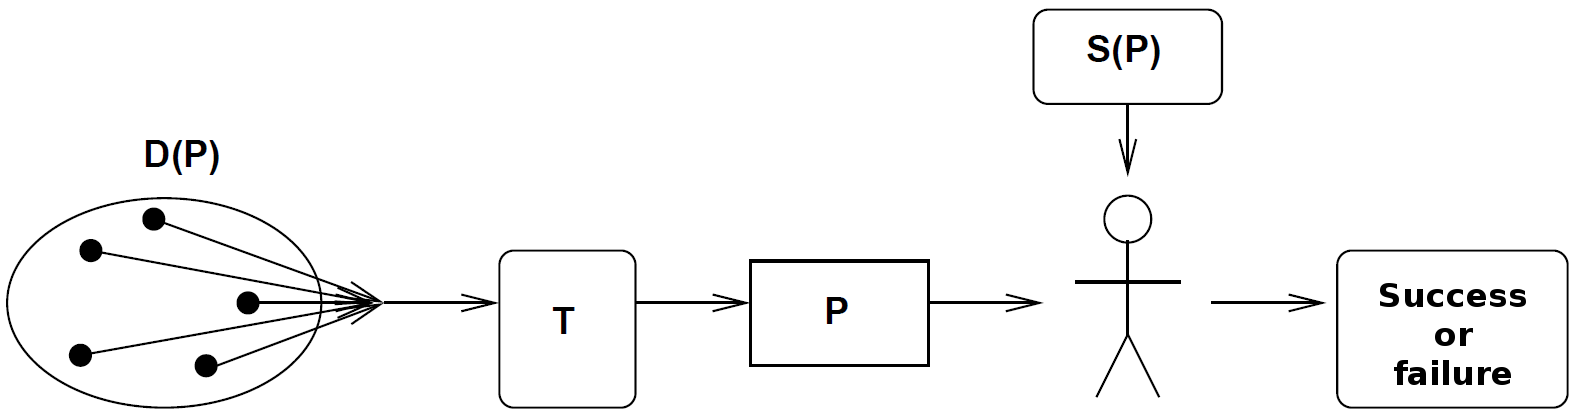
\includegraphics[width=\textwidth]{random-software-testing}
\end{block:fact}
\end{frame}


\begin{frame}
\frametitle{Test technique}
\framesubtitle{Random testing}

\begin{block:concept}{Reliability}
\begin{itemize}
	\item Using random testing, statistical measures of reliability can be
	achieved according to an operational profile.

	\item For every (input data of a) test case, it is assigned a probability
	distribution according to their occurrence in actual operation.
\end{itemize}
\end{block:concept}

\begin{block:fact}{Effectiveness}
\begin{itemize}
	\item It depends on the correctly definition of the operational profile.

	\item If the probability of occurrence of each input data is the same,
	random testing is regarded as the least effective technique for software
	testing~\cite[p. 43]{myers:2004}.
\end{itemize}

\end{block:fact}


\end{frame}


\begin{frame}
\frametitle{Test technique}
\framesubtitle{Partition testing}
\label{concept:partition-testing}

\begin{block:concept}{Definition}
Partition testing is meant any testing scheme which forces execution
of at least one test case from each subset of a partition of the input
domain
\end{block:concept}

\begin{block:fact}{}
    \centering
    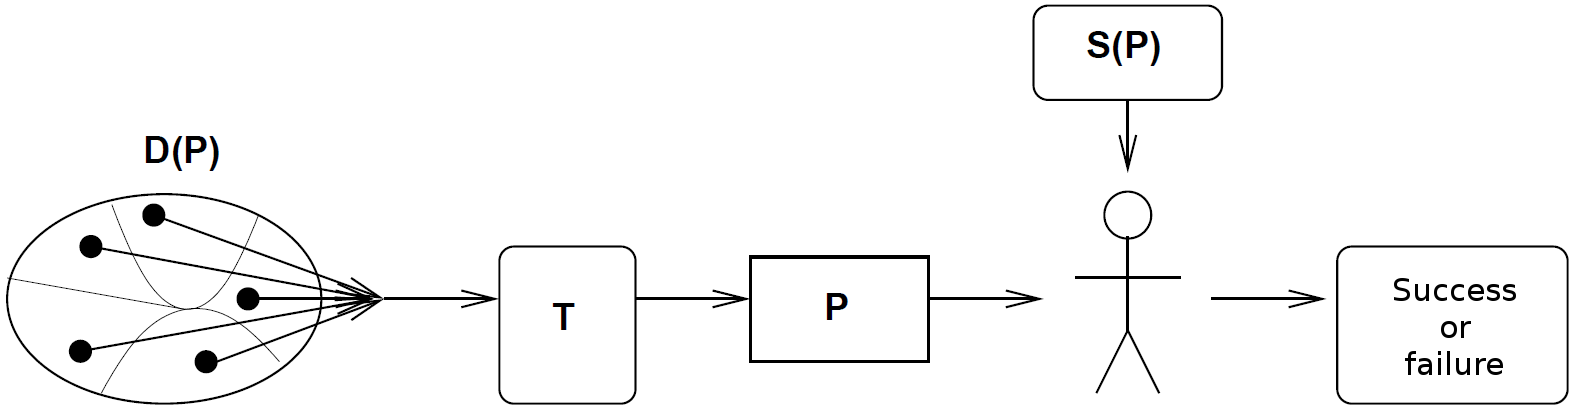
\includegraphics[width=\textwidth]{partition-software-testing}
\end{block:fact}
\end{frame}



\begin{frame}
\frametitle{Test technique}
\framesubtitle{Functional testing}
\label{concept:functional-testing}

\begin{block:concept}{Definition}
Functional testing is a technique based solely on the requirements and
specifications.
\end{block:concept}

\begin{block:fact}{}
\begin{itemize}
	\item Functional testing is also known as black box testing.

	\item Functional testing obtains test requirements from the
	software specification.
	\begin{itemize}
		\item Functional testing requires no knowledge of the internal paths,
		structure, or implementation of the software under test.
	\end{itemize}
\end{itemize}
\end{block:fact}

\hfill
\refie{example:functional-testing}{\beamerbutton{Example}}
\end{frame}


\begin{frame}
\frametitle{Test technique}
\framesubtitle{Functional testing}

\begin{block:fact}{Functional test criteria}
\begin{itemize}
	\item Equivalence partition.
	\item Boundary-value analysis.
	\item Cause-effect graph.
	\item \ldots
\end{itemize}
\end{block:fact}
\end{frame}



\begin{frame}
\frametitle{Test technique}
\framesubtitle{Structural testing}

\begin{block:concept}{Definition}
Structural testing is a technique based on the internal paths, structure,
and implementation of the software under test.
\end{block:concept}


\begin{block:fact}{}
\begin{itemize}
	\item Structural testing is also known as white box testing.

	\item Structural testing obtains test requirements from implementation
	features.
\end{itemize}
\end{block:fact}

\begin{block:fact}{}
    \centering
    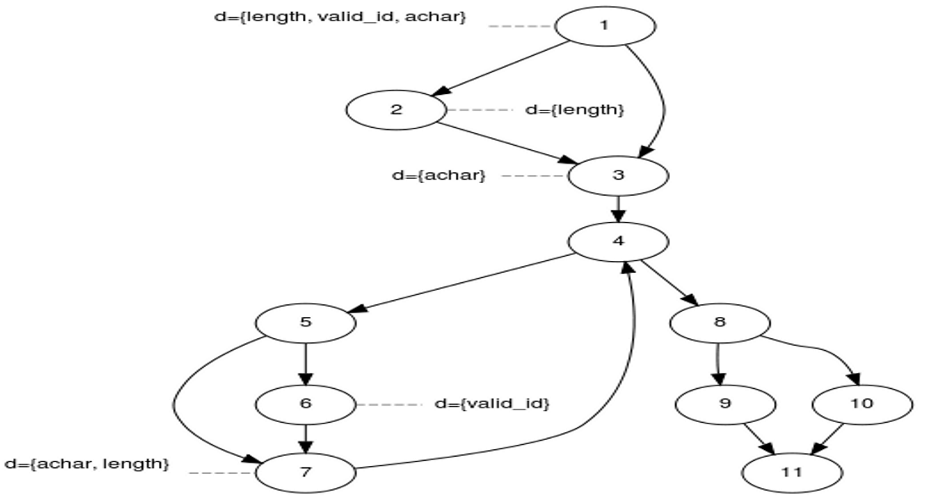
\includegraphics[width=6cm]{structural-testing}
\end{block:fact}
\end{frame}


\begin{frame}
\frametitle{Test technique}
\framesubtitle{Structural testing}
\label{concept:structural-testing-criteria}

\begin{block:fact}{Control-flow based criteria}
\begin{itemize}
	\item Criteria based on the flow of control within a program:
	\begin{itemize}
		\item Statement coverage.
		\item Decision coverage.
		\item Condition coverage.
		\item \ldots
	\end{itemize}
\end{itemize}
\end{block:fact}


\begin{block:fact}{Data-flow based criteria}
\begin{itemize}
	\item Criteria based on the usage of data (variable creation, definition,
	and use):
	\begin{itemize}
		\item All-uses.
		\item All-potential-uses
		\item \ldots
	\end{itemize}
\end{itemize}
\end{block:fact}


\hfill
\refie{example:structural-testing}{\beamerbutton{Example}}
\end{frame}




\begin{frame}
\frametitle{Test technique}
\framesubtitle{Fault-based testing}
\label{concept:fault-based-testing}

\begin{block:concept}{Definition}
Fault-based testing is a technique in which testing is based on
historical information about common faults detected during the software
development life cycle.
\end{block:concept}

\begin{block:fact}{}
    \centering
    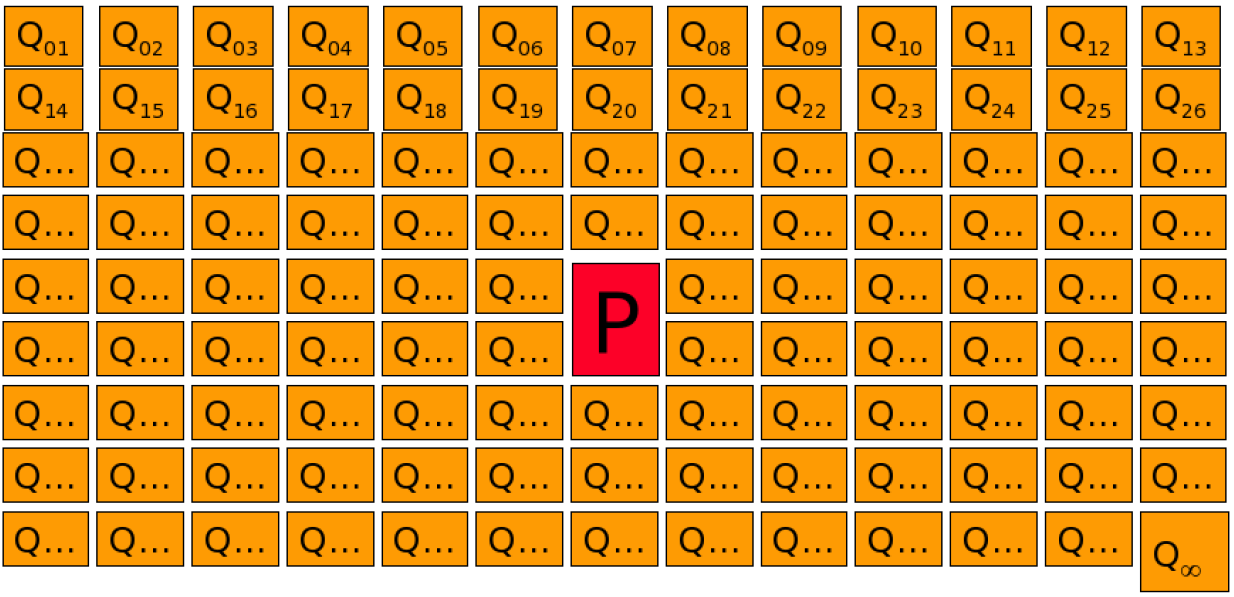
\includegraphics[width=7cm]{mutation-testing}
\end{block:fact}
\end{frame}


\begin{frame}[hasprev=true, hasnext=false]
\frametitle{Test technique}
\framesubtitle{Fault-based testing}
\label{concept:fault-based-test-criteria}

\begin{block:fact}{Fault-based test criteria}
\begin{itemize}
	\item Error seeding.
	\item Mutation:
	\begin{itemize}
		\item Mutation analysis.
		\item Interface mutation.
		\item \ldots
	\end{itemize}
\end{itemize}
\end{block:fact}

\hfill
\refie{example:fault-based-testing}{\beamerbutton{Example}}
\end{frame}


\subsection{Software testing process}
\begin{frame}[parent={cmap:software-testing-foundations}, hasprev=false, hasnext=true]
\frametitle{Software testing process}
\label{concept:software-testing-process}
\label{concept:test-process}

\begin{block:fact}{Software testing process}
\begin{itemize}
	\item When conducted in a systematic and clear-sighted way, software
	testing helps to:
	\begin{itemize}
		\item Increase confidence that the product behaves according to its
		specification.

		\item Highlight minimal characteristics of product quality.
	\end{itemize}
\end{itemize}
\end{block:fact}
\end{frame}


\begin{frame}[hasprev=true, hasnext=false]
\frametitle{Software testing concepts}
\framesubtitle{Software testing}

\begin{figure}
	\centering
	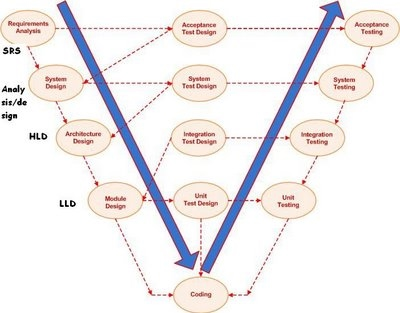
\includegraphics[width=8cm]{figs/v-model}
\end{figure}
\end{frame}


\part{References and credits}
\backmatter{}
\part{References}
\section*{References}


\begin{frame}[label=references, allowframebreaks]{\refname}
\bibliographystyle{abnt-num}
\bibliography{root}
\end{frame}

\part{Acknowledgement}
\section*{Acknowledgement}


\begin{frame}[c,label=credits]
\frametitle{Credits}

\begin{itemize}
	\item Reviewers:
	\begin{itemize}
		\item Marcio Eduardo Delamaro
	\end{itemize}
\end{itemize}
\end{frame}



\part{Instructional elements}
\section{Examples}


% Structural software testing
%
\part{Structural software testing}
\subsection{Control flow graph}
\insertexample{identifier-cfg}{concept:cfg-graph-elements}

\subsection{Definition-use graph}
\insertexample{program-graph}{concept:definition-use-graph}

\subsection{Identifier definition-use graph}
\insertexample{identifier-dug}{concept:definition-use-graph}


% Path
%
\part{Path}
\subsection{Infeasible path}
\insertexample{identifier-infeasible-path}{concept:infeasible-path}

\subsection{Complete path}
\insertexample{identifier-complete-path}{concept:complete-path}

\subsection{Definition-clear paths example}
\insertexample{identifier-def-clear-path}{concept:definition-clear-path}


% Control flow test criterion
%
\part{Control-flow based testing}
\subsection{All-nodes}
\insertexample{all-nodes}{concept:all-nodes}

\subsection{All-paths infeasibility}
\insertexample{all-paths}{concept:all-paths}


% Complexity-based test criterion
%
\part{Complexity-flow based testing}
\subsection{McCabe example}
\insertexample{mccabe}{procedure:mccabe-criterion}


% Data flow test criterion
%
\part{Data-flow based testing}
\subsection{All-Uses for Identifier}
\insertexample{identifier-all-uses}{concept:all-uses}

\subsection{All-Pot-Uses for Identifier}
\insertexample{identifier-all-pot-uses}{concept:all-pot-uses}

\section{Exercises}


\end{document}
